\documentclass[10pt]{ctexbeamer}
%\usetheme[block=fill, sectionpage=none]{metropolis}
\usetheme{Copenhagen}
\useinnertheme{circles}

%\setCJKsansfont{FandolFang-Regular} 
\setCJKsansfont{Source Han Sans CN Light}
\setsansfont{Times New Roman}
%\useoutertheme{infolines}
%\usecolortheme{custom2}
%\useinnertheme{metropolis}
\usepackage{listings}
\usepackage{tikz}
\usetikzlibrary{calc, shapes, backgrounds}
\usepackage{amsmath, amssymb}
\usepackage{xcolor}
\usepackage{color}
\lstset{
    basicstyle=\ttfamily\small,
    columns=fixed,       
    numbers=left,                                        % 在左侧显示行号
    frame=none,                                          % 不显示背景边框
    backgroundcolor=\color[RGB]{245,245,244},            % 设定背景颜色
    keywordstyle=\color[RGB]{40,40,255},                 % 设定关键字颜色
    numberstyle=\footnotesize\color{darkgray},           % 设定行号格式
    commentstyle=\it\color[RGB]{0,96,96},                % 设置代码注释的格式
    stringstyle=\slshape\color[RGB]{128,0,0},   % 设置字符串格式
    showstringspaces=false,                              % 不显示字符串中的空格
    language=c++,                                        % 设置语言
    tabsize=4
}


  
\usepackage{appendixnumberbeamer}

\usepackage{booktabs}
\usepackage[scale=2]{ccicons}

\usepackage{pgfplots}
\usepackage{ulem}
\usepackage{caption}
\usepgfplotslibrary{dateplot}
\usepackage{xspace}
\newcommand{\themename}{\textbf{\textsc{metropolis}}\xspace}
\usepackage{makecell}
\title{zip}
\subtitle{雷达感知数据高效压缩工具的设计与实现}
\date{\today}
\author{报告人:陈建帅,指导老师:张海滨}
\institute{BUPT}
\titlegraphic{\hfill\includegraphics[height=1.5cm]{figures/xiaohui.png}}

\begin{document}
\frame[plain,noframenumbering]{\titlepage}


%------------------目录页
\begin{frame}           %生成目录页,目录太长时加选项[shrink]
  %	\setcounter{page}{0}	%setcounter似乎对beamer无效
    \addtocounter{framenumber}{-2}%---------位置放在beginframe之后,不然无效
    \frametitle{目录}
    \thispagestyle{empty}
    \tableofcontents        % 也可以插入选项 [pausesections]
    %----------------------列目录时,隐藏所有的小节
    %\tableofcontents[hideallsubsections]
\end{frame}

\section{题目}
\subsection{背景}
\begin{frame}{雷达感知数据高效压缩工具的设计与实现}
  在智慧交通系统的边缘计算设备上,需要保存大量的雷达感知历史数据,原始数据的规模非
常大,不加压缩的存储会带来较大的硬件成本。当前,已经有很多优秀的通用压缩算法及其实
现,比如 gzip,bzip2 等。他们可以针对任意形式的文件或者数据进行压缩,通用性和压缩率
都非常优秀。但是,雷达感知数据具有较明显的特点,如果我们可以实现针对此类数据的、更高
效的压缩算法,就可以节约大量存储空间、节省边缘计算设备的算力,带来经济成本优势。
\end{frame}
\subsection{数据特点}
\begin{frame}{数据特点}
  这些数据主要以 json 格式存储,一个非常明显的特点就是:json 的关键字会产生
大量重复。而且,json 格式一般以 ascii 码存储,字符集仅为 128,只需要 7bit 就可以
存储一个字符。利用好这些特点,才能设计出更好的专用压缩工具。
\end{frame}
\section{方案}
\subsection{开发环境}
\begin{frame}{environment}
  \begin{itemize}
    \item 操作系统:linux。考虑到智慧系统边缘计算设备的环境,和现有条件,选择manjaro linux系统进行开发。
    \item 语言:c++17。
    \item 测试:gtest。GoogleTest is Google’s C++ testing and mocking framework. 
    \item 性能分析工具:Clion自带的。可视化和调用列表非常清晰。
  \end{itemize}
\end{frame}
\subsection{整体流程(AC->zlib->Huffman)}
\begin{frame}{PipeLine}
  输入->AC自动机匹配->匹配结果编码->zlib压缩->Huffman编码->输出
\end{frame}
\begin{frame}{AC自动机}
  \ \ \ \ 通过观察雷达感知数据,可以发现有大量重复的字段。比如\text{\{"x":}、\text{"type":"bbox","device":"}等。
  我们可以考虑\textbf{多模匹配算法:AC自动机}。

  \ \ \ \ 给定模式串集合$\{s_1,s_2,\dots s_n\}$和文本串$S$,Automaton可以找出匹配串在文本串的所有位置。可以说是一种在trie树上的KMP算法。

\end{frame}

\begin{frame}{AC自动机的时间复杂度}
其时间复杂度非常优秀:
\begin{block}{时间复杂度}
  定义 $|s_i|$ 是模式串的长度,$|S|$ 是文本串的长度,$|\Sigma|$ 是字符集的大小(在我们的问题中是128)。如果连了 trie 图,时间复杂度就是 $O(\sum|s_i|+n|\Sigma|+|S|)$,其中 $n$ 是 AC 自动机中结点的数目,并且最大可以达到 $O(\sum|s_i|)$。如果不连 trie 图,并且在构建 fail 指针的时候避免遍历到空儿子,时间复杂度就是 $O(\sum|s_i|+|S|)$。
\end{block} 
\end{frame}

\begin{frame}{Automaton}
  模式串集合\texttt{i\ hers\ his\ she}构成的trie树。
  \begin{figure}[!h]
    \centering
    \includegraphics[width=0.9\textwidth]{../pictures/ac-automaton4.png}
    \caption{Automaton}
  \end{figure}
\end{frame}

\begin{frame}{zlib}
  现有很多开源代码实现了gzip等压缩算法,比如zlib头文件。它使用C语言实现了gzip的相关算法(如deflate等)。
  借助这些工具,可以提升我们雷达数据压缩工具的性能。
  \begin{itemize}
    \item \texttt{ZEXTERN int ZEXPORT compress OF((Bytef *dest,   uLongf *destLen, const Bytef *source, uLong sourceLen));}\\
      将source数组中长度为sourceLen的内容\textbf{压缩至}dest数组中,压缩后的长度写入\textbf{destLen指针}。
    \item \texttt{ZEXTERN int ZEXPORT uncompress OF((Bytef *dest,   uLongf *destLen, const Bytef *source, uLong sourceLen));}\\
    将source数组中长度为sourceLen的内容\textbf{解压缩至}dest数组中,解压缩后的长度写入\textbf{destLen指针}。
  \end{itemize}
\end{frame}

\begin{frame}{encode}
  在进行程序设计时,通常给每一个字符标记一个单独的代码来表示一组字符,即\textbf{编码}。

在进行二进制编码时,假设所有的代码都等长,那么表示 $n$ 个不同的字符需要 $\left \lceil \log_2 n \right \rceil$ 位,称为 \textbf{等长编码}(ASCII编码就是一种典型的等长编码,$n=128,\left \lceil \log_2 n \right \rceil = 7$)。

如果每个字符的 使用频率相等,那么等长编码无疑是空间效率最高的编码方法,而如果字符出现的频率不同,则可以让频率高的字符采用尽可能短的编码,频率低的字符采用尽可能长的编码,来构造出一种\textbf{不等长编码},从而获得更好的空间效率。

\end{frame}
\begin{frame}{Huffman}

在设计不等长编码时,要考虑解码的唯一性,如果一组编码中任一编码都不是其他任何一个编码的前缀,那么称这组编码为 前缀编码,其保证了编码被解码时的唯一性。

霍夫曼树可用于构造 最短的前缀编码,即 \textbf{霍夫曼编码(Huffman Code)}
\end{frame}

\begin{frame}{Huffman}
 霍哈夫曼编码构造步骤如下:
\begin{enumerate}
  \item 设需要编码的字符集为:$d_1,d_2,\dots,d_n$,他们在字符串中出现的频率为:$w_1,w_2,\dots,w_n$。
  \item 以 $d_1,d_2,\dots,d_n$ 作为叶结点,$w_1,w_2,\dots,w_n$ 作为叶结点的权值,构造一棵霍夫曼树。
  \item 规定哈夫曼编码树的左分支代表 $0$,右分支代表 $1$,则从根结点到每个叶结点所经过的路径组成的 $0$、$1$ 序列即为该叶结点对应字符的编码。
\end{enumerate}
\end{frame}

\begin{frame}{Huffman}
\begin{columns}
  \column{0.5\textwidth}
  \tikzset{
  left/.style = {fill = orange!90!blue},
  right/.style = {fill = blue!70!yellow}
}
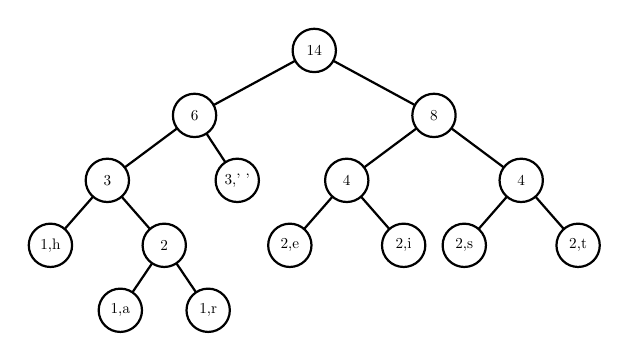
\begin{tikzpicture}[
  scale = 0.55, transform shape, thick,
  every node/.style = {draw, circle, minimum size = 10mm},
  grow = down,  % alignment of characters
  level 1/.style = {sibling distance=4.5cm},
  level 2/.style = {sibling distance=3cm}, 
  level 3/.style = {sibling distance=1.6cm}, 
  level 4/.style = {sibling distance=1cm}, 
  level distance = 1.5cm
]
% \node[fill = gray!40, shape = rectangle, rounded corners,
%   minimum width = 6cm, font = \sffamily] {Coin flipping} 
\node[](root){14}
child{node[left](B1){6}
  child{node[left](C1){3}
    child{node[left](D1){1,h} }
    child{node[right](D2){2}
      child{node[left](E1){1,a}}
      child{node[right](E2){1,r}}
    }
  }
  child{node[left](C2){3,' '}}
}
child{node[right](B2){8}
  child{node[left](C3){4}
    child{node[left](D3){2,e}}
    child{node[right](D4){2,i}}
  }
  child{node[right](C4){4}
    child{node[left](D5){2,s}}
    child{node[right](D6){2,t}}
  }
};
% \node[shape = circle split, draw, line width = 1pt,
%         minimum size = 10mm, inner sep = 0mm, font = \sffamily\large,
%         rotate=30] (Start)
%         { \rotatebox{-30}{H} \nodepart{lower} \rotatebox{-30}{T}}
%  child {   node [head] (A) {}
%    child { node [head] (B) {}}
%    child { node [tail] (C) {}}
%  }
%  child {   node [tail] (D) {}
%    child { node [head] (E) {}}
%    child { node [tail] (F) {}}
%  };

% Filling the root (Start)
% \begin{scope}[on background layer, rotate=30]
%   \fill[head] (Start.base) ([xshift = 0mm]Start.east) arc (0:180:5mm)
%     -- cycle;
%   \fill[tail] (Start.base) ([xshift = 0pt]Start.west) arc (180:360:5mm)
%     -- cycle;
% \end{scope}

% Labels
% \begin{scope}[nodes = {draw = none}]
%   \path (Start) -- (A) node [near start, left]  {$0.5$};
%   \path (A)     -- (B) node [near start, left]  {$0.5$};
%   \path (A)     -- (C) node [near start, right] {$0.5$};
%   \path (Start) -- (D) node [near start, right] {$0.5$};
%   \path (D)     -- (E) node [near start, left]  {$0.5$};
%   \path (D)     -- (F) node [near start, right] {$0.5$};
%   \begin{scope}[nodes = {below = 11pt}]
%     \node [name = X] at (B) {$0.25$};
%     \node            at (C) {$0.25$};
%     \node [name = Y] at (E) {$0.25$};
%     \node            at (F) {$0.25$};
%   \end{scope}
%   \draw[densely dashed, rounded corners, thin]
%     (X.south west) rectangle (Y.north east);
% \end{scope}
  
\end{tikzpicture}
\column{0.5\textwidth}
  文本\texttt{this is a tree}的编码结果是
\texttt{111 000 101 110 01 101 110 01 0010 01 111 0011 100 s100}

\begin{columns}
  \column{0.5\textwidth}
  \begin{table}
    \begin{tabular}{c|c|c}
      char & f & code \\
      \midrule
      space & 3 & 01\\
      a & 1 & 0010\\
      e & 2 & 100\\
      h & 1 & 000\\
    \end{tabular}
  \end{table}
  \column{0.5\textwidth}
  \begin{table}
    \begin{tabular}{c|c|c}
      char & f & code \\
      \midrule
      i & 2 & 101\\
      r & 1 & 0011\\
      s & 2 & 110\\
      t & 2 & 111\\
    \end{tabular}
  \end{table}
\end{columns}
\end{columns}
\end{frame}

\begin{frame}{input/output}
  输入输出采用\texttt{fread/fwrite}系统调用。这要比\texttt{cin/cout}或\texttt{scanf/printf}快很多。

  另外,我们的专用压缩工具现在支持如下选项:
  \begin{figure}[!h]
    \centering
    \includegraphics[width=0.7\textwidth]{./figures/p3.png}
    \caption{options}
  \end{figure}
\end{frame}
\subsection{测试}
\begin{frame}{gtest}
  GoogleTest is Google's C++ testing and mocking framework. 

  例如:霍夫曼编码模块与其他模块并不相关。我们可以单独测试这一模块,通过测试后进行其他模块开发。
\end{frame}

\begin{frame}{profile}
\begin{figure}[!h]
  \centering
  \includegraphics[width=0.95\textwidth]{./figures/flamegraph.png}
  \caption{柱状图}
\end{figure}

如上图,可以看出现有算法的耗时分布。各步骤大体占比如下
\begin{itemize}
  \item AC自动机匹配:28\%
  \item 匹配编码:12\%
  \item zlib压缩:42.86\%
  \item 哈夫曼编码:5.05\%
  \item 输入输出:忽略不计
\end{itemize}

\end{frame}

\begin{frame}{profile}
  下图 为函数调用链上的信息
\begin{figure}[!h]
  \centering
  \includegraphics[width=0.85\textwidth]{./figures/p5_2.png}
  \caption{method}
\end{figure}
\end{frame}

\section{效果对比及下一步优化步骤}
\begin{frame}{result}

  \begin{table}
    \caption{文件1:523582020字节}
    \begin{tabular}{c|c|c|c|c|c}
      \toprule
      \makecell{算法}& \makecell{压缩时间\\(ms)} & \makecell{压缩大小\\(byte)} & 压缩率 & \makecell{速度\\(mb/s)} & \makecell{解压时间\\(ms)}\\
      \hline
      非通用 & 19000 &102813647 &19.64\% & 27.56 &6989.51\\
      \hline
      gzip & 14016 & 94865513 & 18.12\%& 37.56 & 2202\\
      \bottomrule
    \end{tabular}
  \end{table}
\end{frame}
\begin{frame}[fragile]{next step}
  速度上,
  \begin{itemize}
    \item trie树节点的实现。
    
    当前是用指针构建trie树。可以用数组模拟指针,优化耗时。
    \begin{lstlisting}{language=c++}
struct TrieNode {
    TrieNode *nxt[128]{};
    TrieNode *fail;
    int depth;
    int end; 
    char c;
};
        \end{lstlisting}
        我们当前是使用静态的配置文件来生成AC自动机,可以限制配置文件的大小,以限制AC自动机的大小。这样,我们可以使用固定大小的数组模拟堆栈,优化指针寻址耗时。
    \item AC自动机的实现
    
    可以考虑链接trie图,优化时间复杂度。
  \end{itemize}
\end{frame}

\begin{frame}
  {next step}
  压缩率上
  \begin{itemize}
    \item 删除控制符
    
    在匹配结果编码这一步,分控制字符(0/1)和普通编码字符(8bit,模式串占位符和未匹配字符)。但考虑到ascii只有7bit,模式串占位符可以编码128~255,可以省掉控制字符,提升压缩率。

    比如\texttt{0 00110011 1 0000001},0代表后边是ascii字符c,1代表后边是第1个模式串。但如果去掉控制符,可编码为\texttt{00110011 10000001}
    \item 匹配串的选择
    
    当前匹配串并不是最优的。下一步可以思考更好的选择。
  \end{itemize}
\end{frame}
\begin{frame}[fragile]{Thanks}
  谢谢!

  
\end{frame}
\end{document}